Understanding the meaning of \enquote{performance} is key to be able to assess performance portability. 
When we look at the Cambridge Dictionary entry of the word performance, we can see a few different definitions based on the context\footnote{\url{https://dictionary.cambridge.org/dictionary/english/performance}}:
\begin{description}
    \item[activity:] \enquote{how well a person, machine, etc. does a piece of work or an activity}
    \item[entertainment:] \enquote{the action of entertaining other people by dancing, singing, acting, or playing music}
    \item[doing:] \enquote{the act of doing something, such as your job}
    \item[business:] \enquote{how successful an investment, company, etc. is and how much profit it makes}
\end{description}
From these short examples, we can already see that \endquote{a good performance} heavily depends on the context. 
This is also true for performance in the computer science domain. 
For example, when asking Machine Learners about the performance of their \gls{ml} models, they will answer with different model metrics showing how well their model performs on new, unseen data. 
On the other hand, if you ask a member of the \gls{hpc} community about the performance of their, e.g., simulation, you will most likely get an answer regarding the total wall time the simulation needed to complete. 
If I talk about performance in the remainder of this thesis, I will stick to the context of \gls{hpc}. 
However, even in this context, there is no single widely agreed definition or metric to describe the performance of some code. 
Possible metrics can include, but are not limited to:
\begin{description}
    \item[walltime:] Also known as \textbf{runtime} or \textbf{time-to-solution}, the time a code needs to finish its execution.
    \item[throughput:] The rate of finished processing tasks (depending on the problem at hand), an example could be the number of lattice updates.
    \item[scalability:] Does my application demonstrate satisfying strong or weak scaling when increasing the number of available compute resources?
    \item[utilization:] Does my implementation utilize the available compute units to a satisfying degree?
    \item[efficiency:] Is my code efficient enough? This can include walltime, but also other metrics like the amount of used memory or energy.
\end{description}

% TODO: nochmal drüber nachdenken
Two things should be noted when looking at the above list. 
First, the transitions between the different metrics are fluent. 
For example, a good compute utilization most likely also means a small walltime. 
Second, when looking at the metrics, most of the time we look at the relative performance of an application with respect to some baseline. 
As an example, if we analyze the energy efficiency of an application, we most likely say that it is X\si{\percent} more or less efficient than some baseline we want to compare our implementation to. 
In this example, it is rather difficult or outright impossible to determine what the absolutely best energy efficiency would be. 

In the remainder of this thesis, I will focus mostly on the \textbf{walltime} and \textbf{efficiency} mainly with respect to the energy efficiency of the code examples when I talk about performance portability. 
Thereby, gathering basic \textbf{walltime} information is possible in a straightforward way with normal tools directly provided by \cpp, as shown in \autoref{code:walltime_measurement}.

\begin{listing}
    \begin{minted}{c++}
auto start = std::chrono::steady_clock::now();

// your heavy computations on the CPU or GPU

auto end = std::chrono::steady_clock::now();
auto walltime = std::chrono::duration_cast<std::chrono::milliseconds>(end - start).count();
    \end{minted}
    \caption{A small example on how to gather the \textbf{walltime} of a code using the \cpp11 \code{std::chrono} library.}
    \label{code:walltime_measurement}
\end{listing}

However, gathering efficiency metrics like energy consumption, but also memory, or compute utilization poses more challenges, especially if we want to get this information in a vendor-independent way for NVIDIA, AMD, and Intel \glspl{gpu} and \glspl{cpu}. 
While all hardware vendors provide some form of gathering this information through custom libraries, collecting all this information in a vendor-independent way is far from trivial since these libraries do not agree to a standardized interface. 
As an example, to gather the total power consumption (since the last driver reload) for NVIDIA, AMD, and Intel \glspl{gpu}, the library functions shown in \autoref{code:vendor_labrier_calls} must be used.

\begin{listing}
    \begin{minted}{c++}
// NVML
unsigned long long power{};  // mJ
nvmlReturn_t errc = nvmlDeviceGetTotalEnergyConsumption(device_handle, &power);

// ROCm SMI library
[[maybe_unused]] std::uint64_t timestamp{};
float resolution{};
uint64_t power{};  // @$\mu$@J
rsmi_status_t errc = rsmi_dev_energy_count_get(device_handle, &power, &resolution, &timestamp);
float value = power * resolution;

// Level Zero
std::uint32_t num_power_domains{ 0 };  // @$\mu$@J
// enumerate all power domains
if (zesDeviceEnumPowerDomains(device_handle, &num_power_domains, nullptr) == ZE_RESULT_SUCCESS) {
    power_handles.resize(num_power_domains);
    if (zesDeviceEnumPowerDomains(device_handle, &num_power_domains, power_handles.data()) == ZE_RESULT_SUCCESS) {
        // we found at least one power domain (can be empty if reading power related counters isn't supported on the device)
        if (!power_handles.empty()) {
            // get the total power consumption of the first power domain
            zes_power_energy_counter_t energy_counter{};
            if (zesPowerGetEnergyCounter(power_handles.front(), &energy_counter) == ZE_RESULT_SUCCESS) {
                uint64_t power = energy_counter.energy;
            }
        }
    }
}
    \end{minted}
    \caption{
    Example library function calls to gather the total power consumption since the last driver reload from an NVIDIA \gls{gpu} using \gls{nvml}, an AMD \gls{gpu} using \gls{rocmsmi}, and Intel \gls{gpu} using Level Zero.
    Note that the respective environments must be initialized beforehand and that the \code{device_handle} points to a supported and available device.}
    \label{code:vendor_library_calls}
\end{listing}

\autoref{code:vendor_library_calls} shows too major problems in gathering such information in a vendor-independent way. 
First, as already mentioned, the \glspl{api} greatly differ between the different vendors. 
For example, using \gls{nvml} collecting the total power consumption can be done in two lines of code, when using Intel's Level Zero on the other hand, we at least need eight lines of code. 
Second, the libraries do not even agree to the same physical unit: While \gls{rocmsmi} and Level Zero both report the total power consumption in \si{\mu\joule}, NVIDIA's \gls{nvml} library reports it in \si{\milli\joule}.

An additional challenge is that for the walltime it may be sufficient to report it once to get the runtime of the whole application, but for, e.g., the energy consumption it is necessary to sample the information during the whole program execution to get more fine-grained information of your application. 

There already exist small and large libraries which solve at least some of these problems. 
However, they are all restricted in one or another way.
For example, the smaller libraries all support only a small subset of the possible hardware I am interested in. 
\cite{araf_verified_2020, leinardi_greenwithenvy_2024, noauthor_gpu_2024, guerreiro_gpgpu_2018} only support NVIDIA \glspl{gpu}, \cite{amd_amd_2024, noauthor_gpu_2023} only support AMD \glspl{gpu}, \cite{noauthor_ricks-lab_2024} supports NVIDIA and AMD \glspl{gpu}, \cite{benoit_courty_mlco2codecarbon_2024} supports NVIDIA and Intel \glspl{gpu}, \cite{noauthor_libgpucounters_2024} supports ARM Immortalis and Mali \glspl{gpu}, and \cite{google_hardwareperfcounter_2022} supports Adreno and Mali \glspl{gpu}.

The larger libraries do support more different hardware, but with one exception they also do not support all hardware I am interested in. 
PAPI~\cite{mucci_papi_1999} supports low-level performance counters to get various information from different \glspl{cpu} as well as NVIDIA and AMD \glspl{gpu}. 
Likwid~\cite{thomas_gruber_likwid_2023} is similar to PAPI in that it also supports low-level performance counters for different hardware. 
Its main focus lies on \glspl{cpu}, but NVIDIA and AMD \glspl{gpu} are also supported although officially only in an experimental state. 
The PowerAPI~\cite{fieni_powerapi_2024} is a collection of different tools that can be used to measure and analyze the power consumption of applications. 
It supports \glspl{cpu} and \glspl{gpu} from Intel and NVIDIA \glspl{gpu}. 
VARIORUM~\cite{noauthor_variorum_2024} is the only library that supports generic wrappers around low-level \gls{api} functions for all major \gls{cpu} and \gls{gpu} vendors. 

However, none of these libraries support sampling of hardware information during the whole programming execution. 
Therefore, I wrote my own hardware sampling library \textbf{hws} that also wraps the low-level functions from all major hardware vendors and additionally exposes an easy-to-use sampling interface to be able to automatically gather all necessary information during the whole program execution. 




\newpage
Micro-architecture:
\begin{itemize}
    \item fixed for a core of a given micro-architecture
    \item floating point operation per computer operation ($\frac{flop}{operation}$)
    \begin{itemize}
        \item most of the time, only addition, subtraction, and multiplication counted $\rightarrow$ $\frac{1}{1}$
        \item \gls{fma} ($d = a \cdot b + c$) $\rightarrow$ $\frac{2}{1}$
    \end{itemize}
    \item computer operation per instruction ($\frac{operations}{instruction}$)
    \begin{itemize}
        \item vectorization
        \item scalar $\rightarrow$ $\frac{1}{1}$
        \item AVX-512 FP64 $\rightarrow$ $\frac{8}{1}$
    \end{itemize}
    \item instructions per cycle ($\frac{instructions}{cycle}$)
    \begin{itemize}
        \item superscalar execution
        \item vector units simultaneous with scalar units? $\rightarrow$ most of the time ignored
        \item two \gls{fma} operations simultaneously $\rightarrow$ $\frac{2}{1}$
        \item two scalar operations simultaneously $\rightarrow$ $\frac{2}{1}$
        \item a \gls{fma} followed by a scalar $\rightarrow$ $\frac{3}{2}$
    \end{itemize}
\end{itemize}

Machine-architecture:
\begin{itemize}
    \item cycles per second ($\frac{cycles}{second}$)
    \begin{itemize}
        \item frequency
        \item attention: turbo modes, power saving, thermal throttling, different frequencies for AVX instructions, etc.
        \item use AVX all cre frequencies!
    \end{itemize}
    \item cores per socket ($\frac{cores}{scoket}$)
    \begin{itemize}
        \item hyperthreading adds no new resource $\rightarrow$ hyperthreads don't count
    \end{itemize}
    \item sockets per node ($\frac{scokets}{node}$)
\end{itemize}

Final formula: 

\begin{definition}[\gls{flops} per Node~\cite{dolbeau_theoretical_2018}]
Given the micro-architecture and machine-architecture characteristics of a \gls{cpu}, the theoretical peak \acrfull{flops} for a compute node can be calculated using
$$ \frac{flops}{node} = \frac{flop}{operation} \cdot \frac{operations}{instruction} \cdot \frac{instructions}{cycle} \cdot \frac{cycles}{second} \cdot \frac{cores}{socket} \cdot \frac{sockets}{node} $$
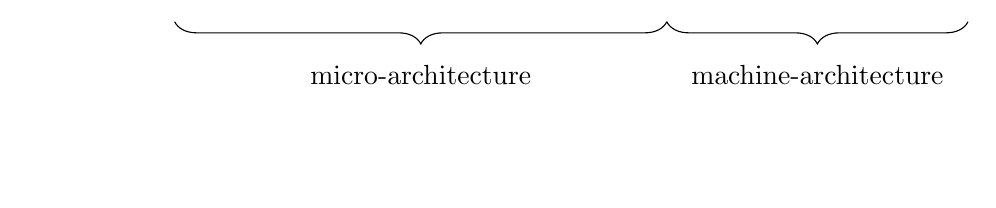
\begin{tikzpicture}
    \node at (0, 0) {}; % dummy node that placement works correctly
    \draw[transform canvas={yshift=1.1cm}, decorate,decoration={brace, amplitude=8pt, mirror, raise=6ex}] (1.75, 0) -- (8, 0) node[midway, yshift=-4.5em]{\text{micro-architecture}};
    \draw[transform canvas={yshift=1.1cm}, decorate,decoration={brace, amplitude=8pt, mirror, raise=6ex}] (8, 0) -- (11.825, 0) node[midway, yshift=-4.5em]{\text{machine-architecture}};
\end{tikzpicture}
\vspace{-1cm}
\end{definition}

non-trivial instructions like division, sqrt, etc.
\begin{itemize}
    \item ignored until now
    \item three cases:
    \begin{enumerate}
        \item source code translates into a single machine instructions with higher-than-normal latency or throughput
        \item source code translates into a fixed number of machine instructions
        \item source code translates into a variable number of machine instructions
    \end{enumerate}
\end{itemize}

Note that all these calculated theoretical peak \gls{flops} only serve as sensible upper-bound. 
It is not guaranteed or even likely that a real-world example will achieve the calculated theoretical peak performance. 
Nevertheless, if all researchers agree on one way to calculate the theoretical peak \gls{flops}, it can be used as a baseline, making results between different papers more easily comparable. 

\todo{how to count flops in a code?!}
\todo{Beispiel stream/triad CPU benchmark + likwid output $\rightarrow$ verifizieren, dass die Berechnung halbwegs sinnvoll ist!}

\url{https://www.netlib.org/benchmark/linpackc.new}
% https://www.netlib.org/benchmark/hpl/HPL_dgemm.html